


\begin{center}
\Huge
	Bevis for cosinusrelationerne
\end{center}

\section*{Cosinusrelationerne}
\stepcounter{section}

\begin{setn}[Cosinusrelationerne]
	\label{setn:cosinusrelationerne}
	For vilkårlige trekanter $\triangle ABC$ som den på Figur \ref{fig:vilkårlig} har vi følgende sammenhæng
	mellem sidelængderne og vinklerne i trekanten.
	\begin{align}
	\label{eq:cos1}
	\begin{split}
		c^2 &= a^2 + b^2 - 2ab\cos(\angle C),  \\
		b^2 &= a^2 + c^2 - 2ac\cos(\angle B), \\
		a^2 &= b^2 + c^2 - 2bc\cos(\angle A).
	\end{split}
	\end{align}
\end{setn}

Som det var tilfældet med sinusrelationerne, kan vi også omskrive cosinusrelationerne, så det er nemmere at finde vinklen, hvis vi kun kender sidelængder. Så lyder cosinusrelationerne

\begin{align}
	\label{eq:cos2}
	\begin{split}
	\cos(\angle C) &= \frac{a^2 + b^2 - c^2}{2ab},\\
	\cos(\angle B) &= \frac{a^2 + c^2 - b^2}{2ac},\\
	\cos(\angle A) &= \frac{b^2 + c^2 - a^2}{2bc}.
	\end{split}
\end{align}

\begin{figure}[H]
	\centering
	\begin{tikzpicture}
		\draw[color = olive, thick] (0,0) -- (5,0) node[midway, anchor = north] {$b$};
		\draw[color = olive, thick] (0,0) -- (4,3) node[midway, anchor = south east] {$c$};
		\draw[color = olive, thick] (5,0) -- (4,3) node[midway, anchor = west] {$a$};
		\node[color = olive, anchor = east] at (0,0) {$A$};
		\node[color = olive, anchor = west] at (5,0) {$C$};
		\node[color = olive, anchor = south] at (4,3) {$B$};
	\end{tikzpicture}
	\caption{Vilkårlig trekant $\triangle ABC$}
	\label{fig:vilkårlig}
\end{figure}
\newpage

\subsection*{Bevis}
Vi skal bevise cosinusrelationerne. Dette gøres ad to omgange; én hvor $\angle C$ er spids og én hvor 
$\angle C$ er stump. Vi starter med at betragte det spidse tilfælde og ser derfor på den første trekant på  Figur \ref{fig:cosbevis}.
\begin{figure}[H]
	\centering
	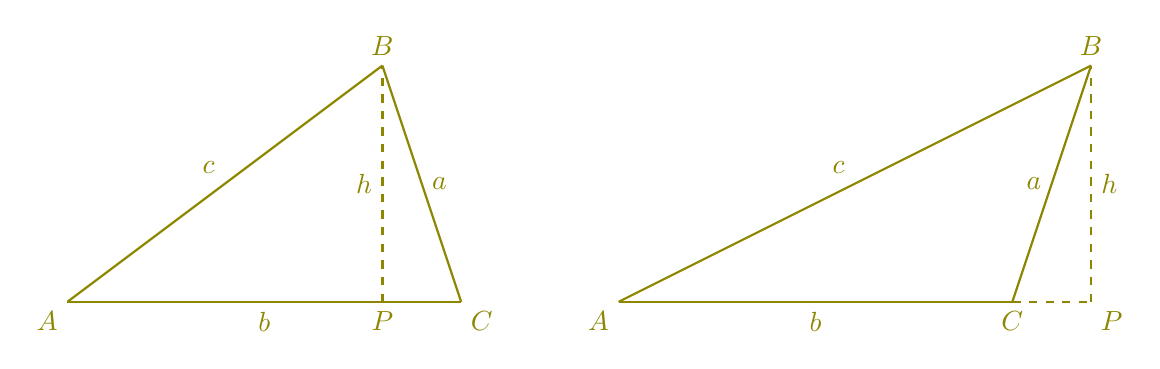
\begin{tikzpicture}
	%Trekant1
	\draw[color = olive, thick] (0,0) -- (5,0) node[midway, anchor = north] {$b$};
	\draw[color = olive, thick] (0,0) -- (4,3) node[midway, anchor = south east] {$c$};
	\draw[color = olive, thick] (4,3) -- (5,0) node[midway, anchor = west] {$a$};
	\draw[color = olive, thick, dashed] (4,0) -- (4,3) node[midway, anchor = east] {$h$};
	\node[color = olive, anchor = north east] at (0,0) {$A$};
	\node[color = olive, anchor = north west] at (5,0) {$C$};
	\node[color = olive, anchor = south] at (4,3) {$B$};
	\node[color = olive, anchor = north] at (4,0) {$P$};
	%Trekant2
	\draw[color = olive, thick] (7,0) -- (12,0) node[midway, anchor = north] {$b$};
	\draw[color = olive, thick] (7,0) -- (13,3) node[midway, anchor = south east] {$c$};
	\draw[color = olive, thick] (13,3) -- (12,0) node[midway, anchor = east] {$a$};
	\draw[color = olive, thick, dashed] (13,0) -- (13,3) node[midway, anchor = west] {$h$};
	\draw[color = olive, thick, dashed] (12,0) -- (13,0);
	\node[color = olive, anchor = north east] at (7,0) {$A$};
	\node[color = olive, anchor = north] at (12,0) {$C$};
	\node[color = olive, anchor = south] at (13,3) {$B$};
	\node[color = olive, anchor = north west] at (13,0) {$P$};
	\end{tikzpicture}
	\caption{Trekanter til bevis af cosinusrelationerne}
	\label{fig:cosbevis}
\end{figure}

\begin{enumerate}[label=\roman*)	]
	\item Hvor langt er linjestykket $PC$ i trekanten $\triangle PBC$? \\ (Vink: Brug formlen
	 $\cos(\angle C) = \frac{\textnormal{hos}}{\textnormal{hyp}})$)
	 \item Hvis linjestykket $AC$ har længde $b$, hvor langt er linjestykket $AP$ så? Brug dit svar fra i).
	 \item Anvend Pythagoras' sætning på trekanten $\triangle ABP$.
	 \item Hæv nu parentesen. (Vink: Husk at bruge en kvadratsætning).
\end{enumerate}
Vi er nu næsten færdige. Vi skal blot vise, at $h^2 + \cos(\angle C)^2a^2 = a^2$
\begin{enumerate}[label=\roman*)]
	\setcounter{enumi}{4}
	\item Anvend Pythagoras' sætning på trekanten $\triangle PBC$ og sammenlign med resultatet fra iv).
\end{enumerate}
Vi skal nu bevise cosinusrelationerne i det tilfælde, at $\angle C$ er stump. Vi betragter derfor den anden trekant på Figur \ref{fig:cosbevis}.

\begin{enumerate}[label=\roman*)]
	\item Hvor langt er linjestykket $CP$ i trekanten $\triangle CBP$? \\
	(Vink: Brug samme formel som tidligere.)
	\item Hvor langt er linjestykket $AP$?
	\item Anvend Pythagoras sætning på trekanten $\triangle ABP$.
	\item Hæv parentesen. (Vink: Husk at bruge en kvadratsætning).
	\item Udnyt, at $\cos(180 - v) = -\cos(v)$.
	\item Sæt firkanten.
\end{enumerate}

